\section{Methodology}

\subsection{Time execution}

The main purpose of time execution comparison in this paper is to deliver results of hypothetical runtime
improvements between the single threaded application, C++ standard execution policies and the custom
implementation described in the \fullref{sec:parallel_for}. Therefore described methods are
benchmarked with the usage of the same hardware. Moreover, several threads configuration are tested
in the case of custom implementation. The expected best performance is to be available around
the number of available hardware threads.

At the listing \ref{lst:timer_interface} there is presented timer class used to measure execution of DWT
processing chain. It is written in RAII format, i.e. Resource Acquisition Is Initialization. RAII is 
popular modern C++ idiom to control the lifetime of the object, e.g. it is used for scope based
dynamic memory management wrappers. Another use case is control of locking and unlocking mechanisms such
as mutexes. The C++ standard library implements such resource managers in a similar way. One action
is taken upon construction time of the object, i.e. in its constructor and the opposite procedure
takes place during destruction process. This approach enables possibility of time measurement automatization.
Firstly, time is measured at the end of initialization process to avoid overhead of constructing helper
objects. Secondly, such measurement takes place at the beginning of the destruction handling for
very similar reason \cite{cppreference}.

Class ``std::chrono::high\_resolution\_clock'' is aimed to represent time measurement mechanism with the
smallest tick period that is provided by certain implementation of the standard C++ library. Usually
the compiler vendors implement this entity as an alias of ``std::chrono::system\_clock'' or
``std::chrono::steady\_clock'', or another independent clock \cite{cppreference}. In the case of used implementation,
i.e. gcc's libstdc++, it is an alias of ``std::chrono::system\_clock''. Such decision is dictated by
the need of using so called wall-clock time \cite{cppreference}.

Elapsed real time or wall-clock time is the actual time that is needed to take from the start of a given
computer program to its end. It can be understood as a difference between the time when a certain task 
finishes and the time when that task started running \cite{wall_clock}. Wall time is thus distinguishable
from CPU time. The latter one measures only the time during active work on given task is performed by the
processor. This difference comes from architecture and runtime dependent factors. For example, it can involve
intentional delays and waiting for availability of certain system resources. It can be better understood
in the following example. Take into consideration mathematical script which results in producing such report:
``Measured CPU time: 0.09s and wall-time: 5m 20.36s''. For over 5 minutes this program was active and during
that time the processor spent only fraction of second performing mathematical operations. Therefore it was
found to be suitable solution in the concurrent execution of DWT processing chain.

At the listing \ref{lst:timer_specializations} there are depicted several template specializations for
handling different types of measurements. The user of this class can specify the accuracy with the C++ standard
aliases for time primitives. If there is need for such low unit of time as nanoseconds, the actual time
is returned to the user in the bigger format. This approach is a convenient way of handling time measurement
for this particular application.

\begin{listing}[!htb]
\begin{minted}[linenos, breaklines]{cpp}
#include <chrono>
#include <fstream>
#include <iostream>

template<typename T = std::chrono::milliseconds>
class Timer {
public:
    using clock = std::chrono::high_resolution_clock;

    Timer() : ostream_{std::cout} {}
    explicit Timer(std::ofstream& fileStream) : ostream_{fileStream} {}
    explicit Timer(const std::string& filepath) :
        fileStream_{filepath, std::ios::app},
        ostream_{fileStream_} {}

    ~Timer() {
        StopTimer();
    }
    Timer(const Timer& other) = delete;
    Timer& operator=(const Timer& other) = delete;
    Timer(Timer&& other) = delete;
    Timer& operator=(Timer&& other) = delete;

private:
    std::ofstream fileStream_{};
    std::ostream& ostream_;
    std::chrono::time_point<clock> startTimePoint_{clock::now()};

    void StopTimer() {
        const auto endTimePoint = clock::now();
        const auto start = std::chrono::time_point_cast<T>(startTimePoint_)
                               .time_since_epoch()
                               .count();
        const auto end = std::chrono::time_point_cast<T>(endTimePoint)
                             .time_since_epoch()
                             .count();
        SaveTime(start, end);
    }

    template<typename Count>
    void SaveTime(Count start, Count end);
};
\end{minted}
\caption{Timer.hpp: User interface}
\label{lst:timer_interface}
\end{listing}

\begin{listing}[!htb]
\begin{minted}[linenos, breaklines]{cpp}
template<>
template<typename Count>
void Timer<std::chrono::nanoseconds>::SaveTime(Count start, Count end) {
    ostream_ << "Elapsed time: " << static_cast<double>(end - start) / 1000.0 << " us  \n";
}

template<>
template<typename Count>
void Timer<std::chrono::microseconds>::SaveTime(Count start, Count end) {
    ostream_ << "Elapsed time: " << static_cast<double>(end - start) / 1000.0 << " ms  \n";
}

template<>
template<typename Count>
void Timer<std::chrono::milliseconds>::SaveTime(Count start, Count end) {
    ostream_ << "Elapsed time: " << static_cast<double>(end - start) / 1000.0 << " s  \n";
}

template<>
template<typename Count>
void Timer<std::chrono::seconds>::SaveTime(Count start, Count end) {
    ostream_ << "Elapsed time: " << end - start << " s  \n";
}

template<>
template<typename Count>
void Timer<std::chrono::minutes>::SaveTime(Count start, Count end) {
    ostream_ << "Elapsed time: " << end - start << " min  \n";
}

template<>
template<typename Count>
void Timer<std::chrono::hours>::SaveTime(Count start, Count end) {
    ostream_ << "Elapsed time: " << end - start << " h  \n";
}
\end{minted}
\caption{Timer.hpp: Template specializations}
\label{lst:timer_specializations}
\end{listing}

The measurements took place on the one specific hardware setup. The notebook used in the experiments
is not usually used as reference in the benchmarking process. However, it represents quite well
a day-to-day usage for average person. The specification of this hardware and software setup
is presented below. Processor details are as follows:
\begin{itemize}
    \item Name: AMD Ryzen 2500U with Radeon Vega Mobile Gfx.
    \item Producer: AuthenticAMD.
    \item Number of cores: 4.
    \item Number of threads: 8.
    \item Base clock: 2.0 GHz.
    \item Max boost clock: up to 3.6 GHz.
    \item Total L1 cache: 384 kB.
    \item Total L2 cache: 2 MB.
    \item Total L3 cache: 384 kB.
    \item CMOS: 14 nm.
\end{itemize}
The Random Access Memory (RAM) installed in the notebook has following capabilities:
\begin{itemize}
    \item Installed memory: 8 GB.
    \item Available memory: 6.9 GB.
    \item Configuration of slots: 2 x 4 GB.
    \item Frequency: 2400 Mhz.
    \item System Memory Type: DDR4.
\end{itemize}
The operating system used is Windows 10 Home Edition 21H1, while chosen compiler is gcc 10.3 from MSYS2 distribution.

\subsection{Image compression}

The output of proposed algorithm is set of chosen filter pair and discrete wavelet transform
decomposition. It is necessary to somehow evaluate these results with the real JPEG 2000 encoding
technique. Moreover, it is essential to compare such results with the best possible ones obtained
using mentioned earlier encoder. Therefore Kakadu software was used both as the reference and
validation codec.

However, during the study it was found out that solution described in this thesis poorly chooses
the best possible pair of filters to be applied on the image. To mitigate such inconvenience it
was decided to modify main algorithm. The modification includes storing information of discrete
wavelet decomposition type with every filter under the test. Although such approach results in
the performance hit of proposed solution, it enables basic functionality which is determination
of the more efficient image compression. Described mitigation involves validation at the side of
the actual JPEG 2000 Part 2 compliant codec. The results are gathered and later processed with
the basic statistics methods.

The reference results are acquired in slightly different fashion. The main disadvantage of using
whole JPEG 2000 encoding process is time needed to perform such calculations. The amount of possible
discrete wavelet transform decompositions in product with different filter pairs can exceed the
number of thousand in specific cases. Taking into consideration not small number of test images
it was decided to improve this process by dropping empirically chosen types of transforms. Firstly,
during the experiments it was observed that vast majority of images performs best in terms of
image compression when the level of DWT chain reached number of five. Therefore it was decided to
drop exhaustive search method for smaller ranks. Another observation was made, i.e. the pair of used
filters with the Part 1 compliant decomposition determined the obtained result in the more significant
way than Part 2 compliant discrete wavelet transform chain with the Part 1 filter. Therefore
to greatly optimize runtime of this procedure, filter pairs with the Part 1 decomposition are
checked at first.

Lastly, the gathered results, both from reference and from proposed solution are evaluated and
compared with each other. 

\section{Data sets}

The image data set gathered to evaluate results of the thesis takes its origin from one of
Tilo Strutz's papers \cite{ref_images}. It was used at first to evaluate multiplierless reversible
color transforms. The main purpose of that paper was to propose an entire family of multiplierless
reversible color transforms and investigate their performance in lossless image compression \cite{multiplierless_rct}.
Therefore it was found out to be suitable for the case of this thesis as lossless image compression
on color pictures is applied as well. The examplary elements of the image data set are available at
figures \ref{fig:example_1}, \ref{fig:example_2} and \ref{fig:example_3}. It is worth noticing that only ppm
(portable PixMap) images were selected due to lack of png format support in Kakadu library.

\begin{figure}[!htb]
    \centering
    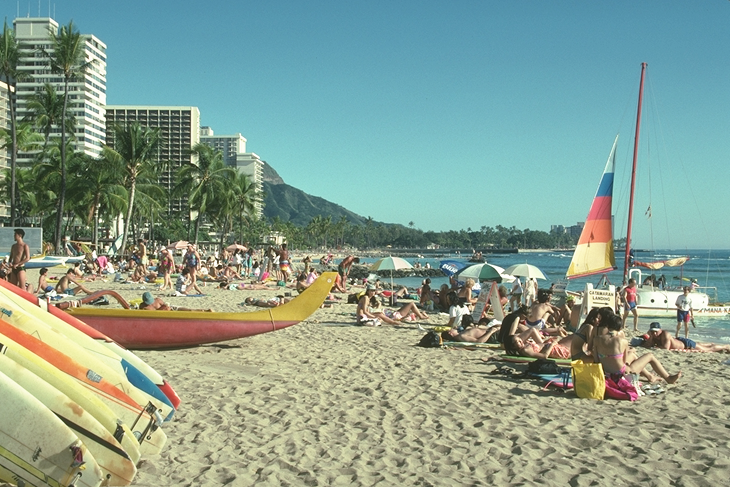
\includegraphics[scale=0.5]{384007.png}
    \caption{The example image from the reference data set \cite{ref_images}}
    \label{fig:example_1}
\end{figure}

\begin{figure}[!htb]
    \centering
    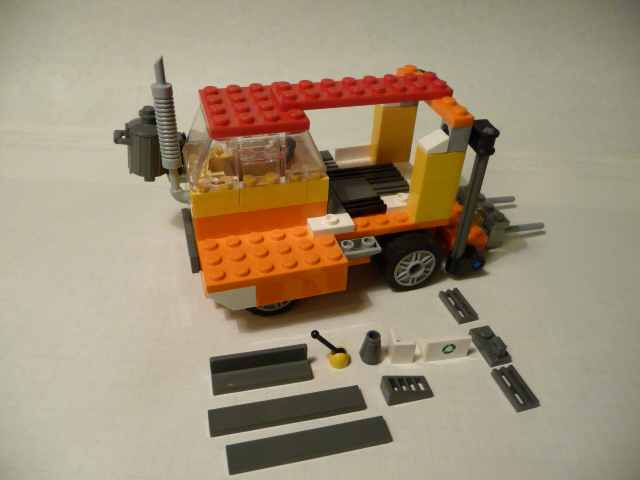
\includegraphics[scale=0.5]{im_0069.png}
    \caption{The example image from the reference data set \cite{ref_images}}
    \label{fig:example_2}
\end{figure}

\begin{figure}[!htb]
    \centering
    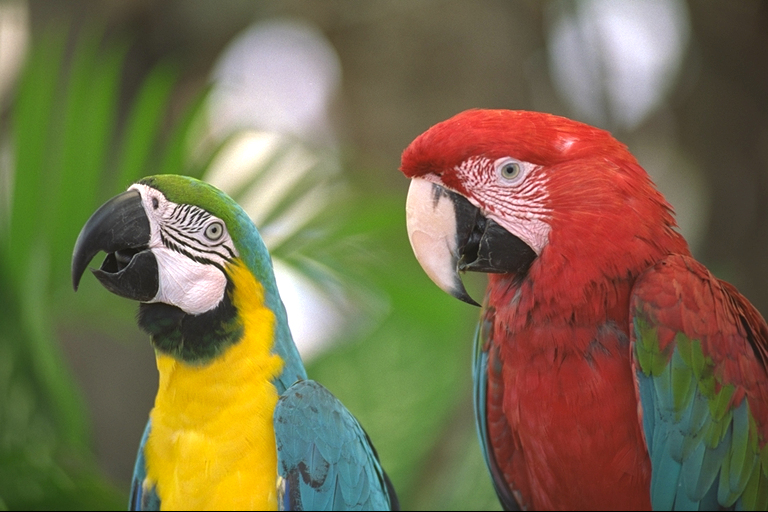
\includegraphics[scale=0.4]{kodim23.png}
    \caption{The example image from the reference data set \cite{ref_images}}
    \label{fig:example_3}
\end{figure}


\section{Results}

\subsection{Reference results} \label{sec:ref_results}

The mean improvement in terms of image compression between Part 1 and Part 2 compliant solutions
turned out to be on average equal to 1.982\% with the standard deviation of 1.307\%. The maximum
possible improvement achieved on specific image was 10.661\% while the minimum was set to 0.

As far as only reference results are concerned it can be concluded that Part 2 extensions such as modification
of discrete wavelet decomposition and change of selected filter pair improve compression ratio
in selected data set. However the results are quite differentiated. For some images the improvement
was significant (over 10\%), while for others there was no improvement. Such behavior probably
involves crash of Kakadu application for certain image.

% mean: -1.9822555180454076
% stddev: 1.3068419882544533
% min: -10.660713840765169
% max: 0.0

\subsection{Estimated best configuration} \label{sec:my_results}

The mean improvement in terms of image compression between Part 1 and Part 2 compliant solutions
turned out to be on average equal to 1.5\% with the standard deviation of 1.305\%. The maximum
possible improvement achieved on specific image was 10.169\% while the minimum was set to 0.

As far as only proposed solution is concerned it can be concluded that Part 2 extensions such as modification
of discrete wavelet decomposition and change of selected filter pair improve compression ratio
in selected data set. However the results are quite differentiated. For some images the improvement
was significant (over 10\%), while for others there was no improvement. Such behavior is present
due to fact that Part 1 solution was used as fallback when no better results were found

% mean: -1.5002908618506086
% stddev: 1.3048358424565147
% min: -10.16940102729851
% max: 0.0

\subsection{Comparison with reference} \label{sec:results_comparison}

Taking into consideration results presented in the \fullref{sec:ref_results} and \fullref{sec:my_results}
it can be stated that they are quite similar. The reference results on average are better by 33\%.
This behavior is expected as the estimation method of proposed solution was memoryless entropy,
while the JPEG 2000 codec has its own memory. Another thing that is worth to notice is that the
choice of filter pair was more important for the final result than the DWT decomposition.
Therefore proposed solution of estimating different shapes of discrete wavelet transform applied
to the image does not guarantee the best possible results. This is due to fact that there was
an impasse on selecting best feasible filter.

\subsection{Time comparison} \label{sec:time_results}

The runtime of discussed solution was measured and later evaluated. Comparison of different
methods at examplary image is presented at the figure \ref{fig:time_comparison_example}. The consecutive
numbers placed after ``thread'' indicate usage of parallel for version presented earlier.
These numbers correspond to number of software threads used in the experiment. The last record, i.e.
``policies'' describes usage of execution policies introduced in C++17. As can be seen at this
figure, selected compiler has not managed to optimize this particular problem. The reason of
this failure may be caused by obscure and non-trivial code. However, proposed version of parallel
computation works as expected. The speedup is strictly connected to the number of hardware threads
which is 8 in this case.

During evaluation process one anomaly was observed (figure \ref{fig:time_comparison_sus}). After investigation
it was concluded that operating system decided to suspend execution of the program due to inactivity.
As can be observed at the figure \ref{fig:time_comparison_means_base} this anomaly higly contributed
to the average measures. It was decided that it has to be eliminated from the data set in the
preprocessing step. At the figure \ref{fig:time_comparison_means_mod} such change is shown.
These results are very similar to the ones presented at first (figure \ref{fig:time_comparison_example}).
The improvement was exhausted around number of hardware threads. Therefore it is not beneficial to
use number of workers greater than hardware concurrency.

\begin{figure}[!htb]
    \centering
    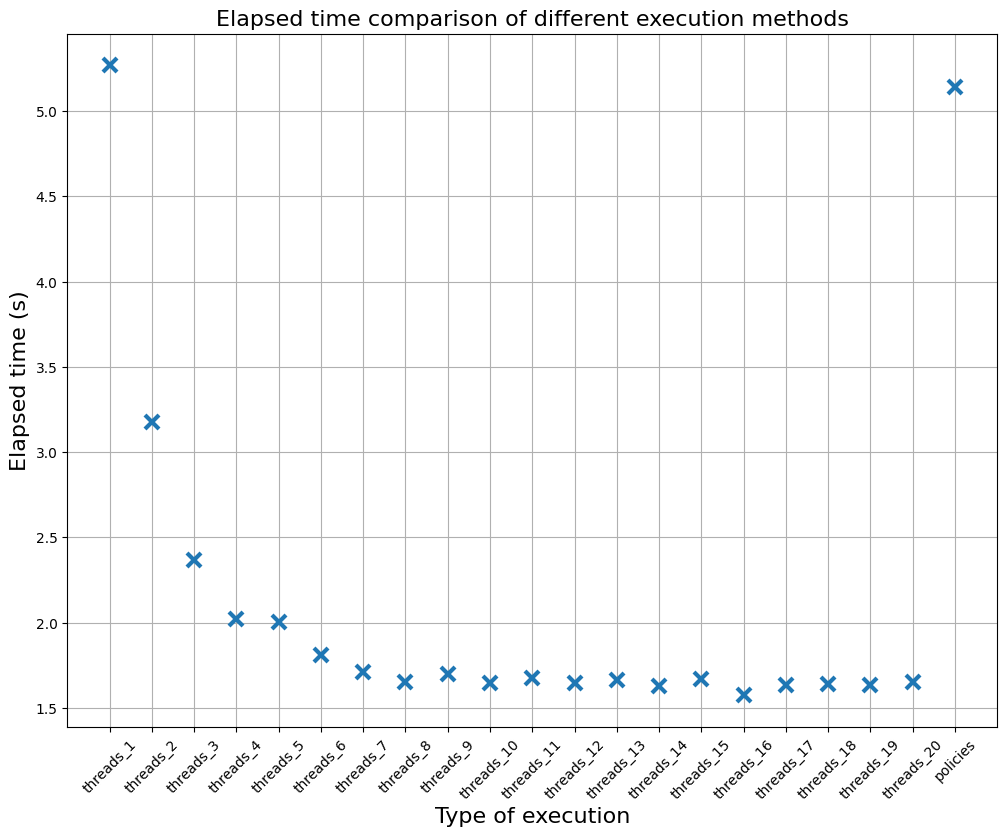
\includegraphics[scale=0.5]{img_0.png}
    \caption{Elapsed time comparison of different execution methods at examplary image}
    \label{fig:time_comparison_example}
\end{figure}

\begin{figure}[!htb]
    \centering
    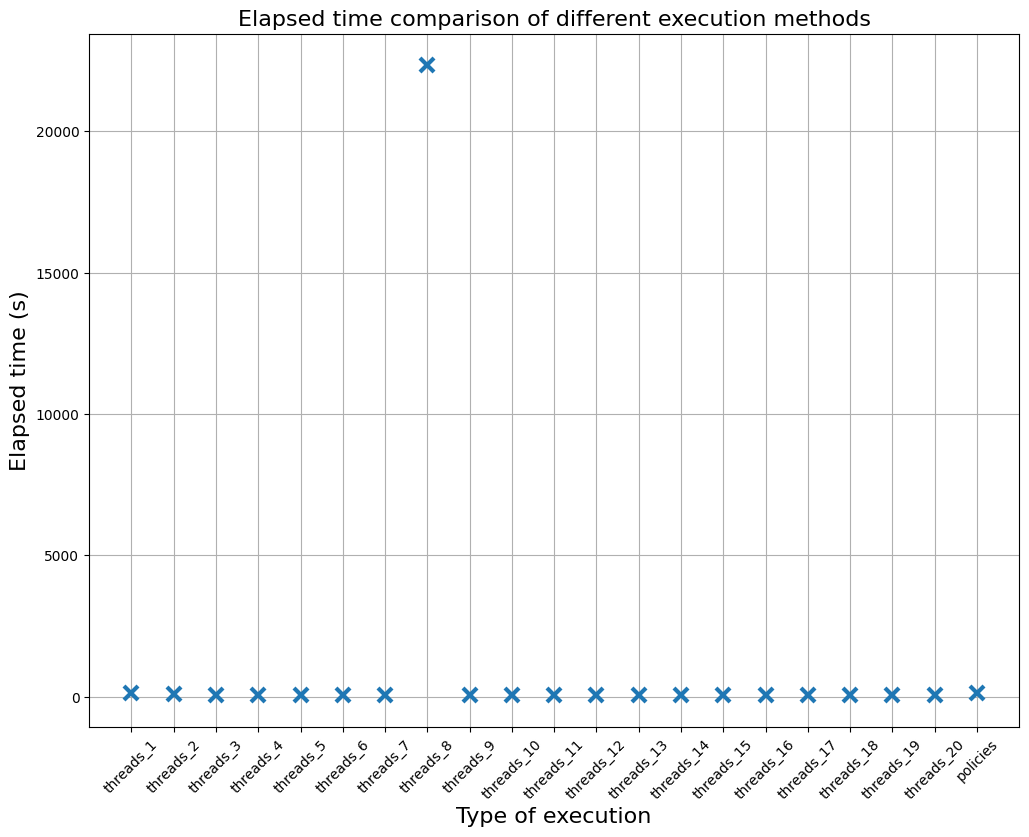
\includegraphics[scale=0.5]{img_73.png}
    \caption{Elapsed time comparison of different execution methods at suspicious run}
    \label{fig:time_comparison_sus}
\end{figure}

\begin{figure}[!htb]
    \centering
    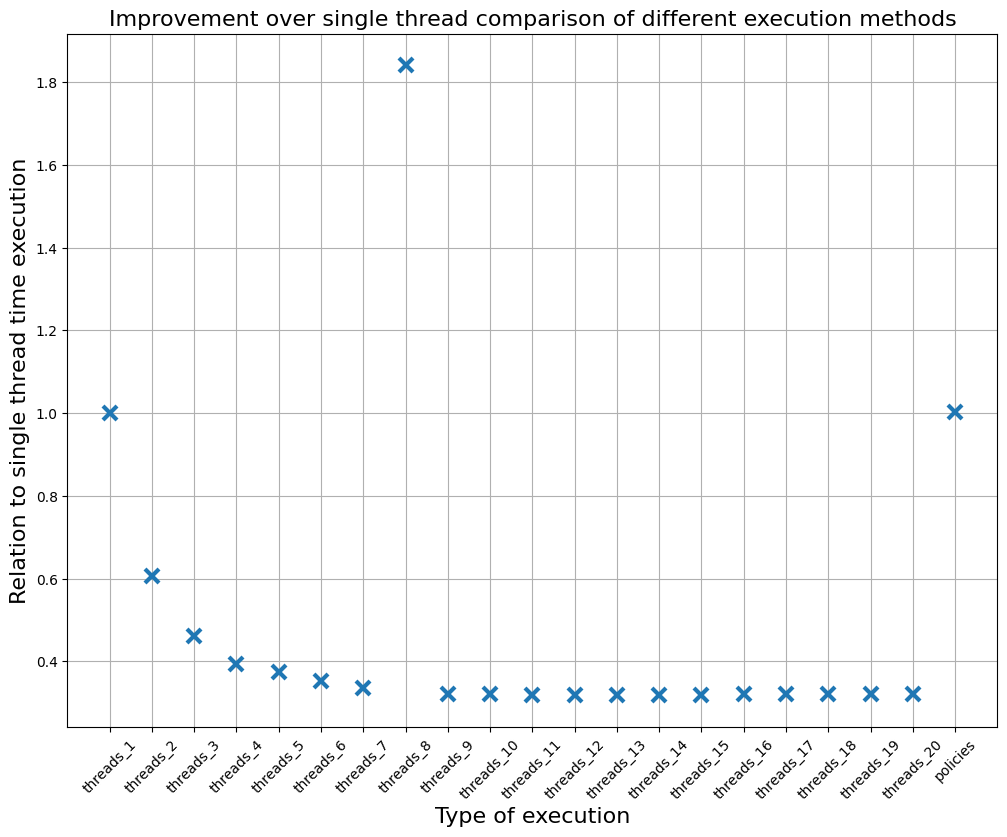
\includegraphics[scale=0.5]{means_base.png}
    \caption{Mean improvement over single thread execution comparison without outliers detection}
    \label{fig:time_comparison_means_base}
\end{figure}

\begin{figure}[!htb]
    \centering
    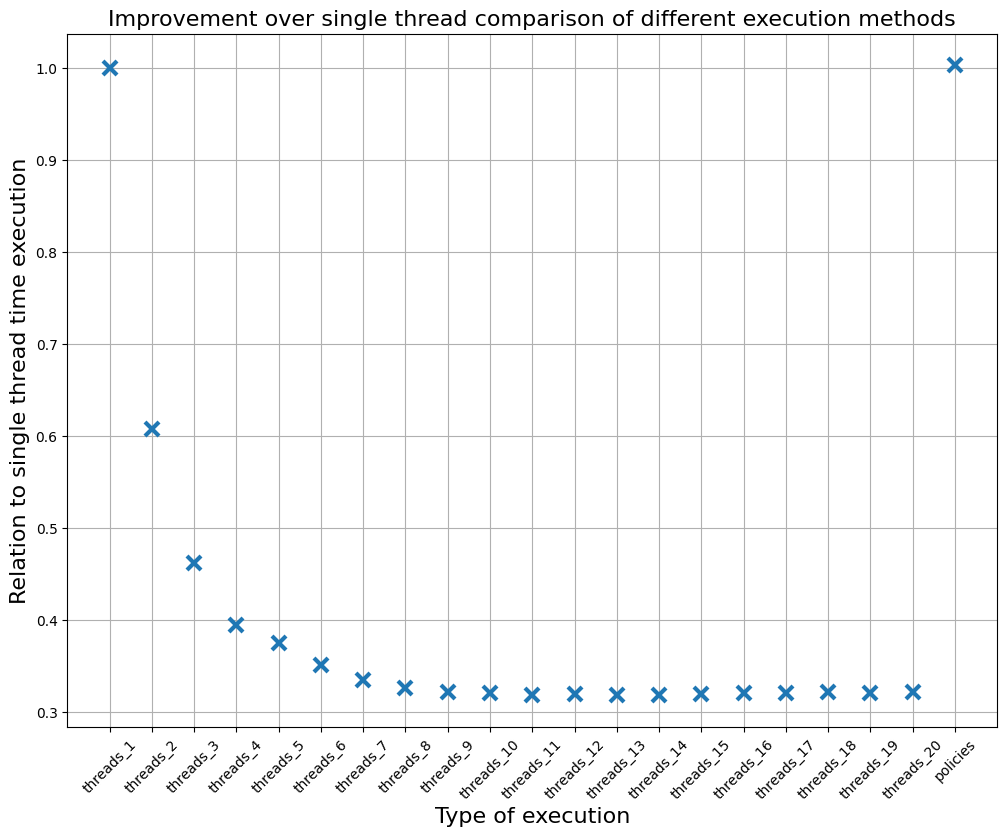
\includegraphics[scale=0.5]{means_mod.png}
    \caption{Mean improvement over single thread execution comparison after outliers removal}
    \label{fig:time_comparison_means_mod}
\end{figure}

\subsection{Visualized sample results}

There are presentend sample outputs of various DWT variants applied to famous 512x512 picture
of Lena Forsén \cite{lena}. All the images are results of low-pass filtering from the last
rank of discrete wavelet transform. The first image \ref{fig:lena_dwt_5} represents the Part 2
compatible decomposition variant where transformation is applied each time only to columns.
Therefore the shape of result is very thin rectangle. Second picture \ref{fig:lena_dwt_199}
illustrates mainly row-wised based DWT.
Another figure \ref{fig:lena_dwt_326} depicts mixed version of discrete wavelet transform described
before. Last one \ref{fig:lena_dwt_363} is the output of Part 1 compliant decomposition.

\begin{figure}[!htb]
    \centering
    
\includegraphics[scale=0.5]{lena_dwt_5.png}
    \caption{The example output image of DWT processing chain using Lena test image \cite{lena}}
    \label{fig:lena_dwt_5}
\end{figure}

\begin{figure}[!htb]
    \centering
    
\includegraphics[scale=1]{lena_dwt_199.png}
    \caption{The example output image of DWT processing chain using Lena test image \cite{lena}}
    \label{fig:lena_dwt_199}
\end{figure}

\begin{figure}[!htb]
    \centering
    
\includegraphics[scale=1]{lena_dwt_326.png}
    \caption{The example output image of DWT processing chain using Lena test image \cite{lena}}
    \label{fig:lena_dwt_326}
\end{figure}

\begin{figure}[!htb]
    \centering
    
\includegraphics[scale=1]{lena_dwt_363.png}
    \caption{The example output image of DWT processing chain using Lena test image \cite{lena}}
    \label{fig:lena_dwt_363}
\end{figure}
